\documentclass[conference,9pt]{IEEEtran}
\usepackage{amsmath,amssymb}
\usepackage{booktabs,array}
\usepackage{graphicx}
\usepackage{tikz}
\usetikzlibrary{arrows.meta,positioning}
\usepackage{cite}
\usepackage{url}
\usepackage{xcolor}
\usepackage[hidelinks]{hyperref}

\newcommand*{\email}[1]{\normalsize\texttt{\href{mailto:#1}{#1}}\par}
\newcommand{\todo}[1]{\textcolor{red}{[TODO: #1]}}
\newcommand{\Bhat}{\widehat{B}}
\newcommand{\Ttwo}{T_2^{\ast}}

% Generated from the frozen confirmation run and the post-hoc analyses; never edit by hand.
% Generated from audited frozen confirmation; do not edit numbers by hand.
\newcommand{\TotalN}{15{,}360}
\newcommand{\NominalHarmCount}{3{,}192}
\newcommand{\NominalHarmRate}{20.78}
\newcommand{\NominalHarmCI}{20.26, 21.30}
\newcommand{\SmallHarmCount}{11{,}510}
\newcommand{\SmallHarmRate}{74.93}
\newcommand{\SmallHarmCI}{74.08, 75.83}
\newcommand{\WeakHarmRate}{99.76}
\newcommand{\WeakReferenceHarmRate}{62.25}
\newcommand{\FallbackCleanRMSE}{6.14}
\newcommand{\ReferenceCleanRMSE}{19.98}
\newcommand{\FallbackAttackRMSE}{23.21}
\newcommand{\ReferenceAttackRMSE}{19.96}
\newcommand{\CleanAlarmRate}{1.07}
\newcommand{\CleanAlarmCI}{0.91, 1.24}
\newcommand{\AbstainAttackN}{296}
\newcommand{\AbstainAttackH}{296}
\newcommand{\AbstainAttackCoverage}{1.93}
\newcommand{\AbstainAttackRisk}{100.00}
\newcommand{\AbstainShotsMillions}{1.04}
\newcommand{\PrimaryHarm}{296}
\newcommand{\ReferenceHarm}{2{,}896}
\newcommand{\GenuineAlarmCount}{154}
\newcommand{\MismatchAlarmRate}{7.68}
\newcommand{\MismatchHarmRate}{1.88}
\newcommand{\HalfHarmRate}{89.67}
\newcommand{\FullHarmRate}{99.98}
\newcommand{\FullAlarmRate}{0.94}
\newcommand{\RunMinutes}{75.6}
\newcommand{\StoredTestCount}{614{,}400}
\newcommand{\StoredCalibrationCount}{737{,}280}
\newcommand{\ArchiveMB}{349.7}
\newcommand{\VerifiedArtifacts}{3{,}213}
\newcommand{\AttackerEvals}{90{,}000}
\newcommand{\SearchStarts}{120}
\newcommand{\EquivalenceError}{5.55\times 10^{-16}}
\newcommand{\FixedU}{14{,}758}
\newcommand{\HiddenU}{1}
\newcommand{\FrequencyU}{14{,}892}
\newcommand{\OptimizedT}{6{,}081}
\newcommand{\OptimizedU}{17}
\newcommand{\MeanU}{14}
\newcommand{\CleanDifference}{-13.84}
\newcommand{\CleanDifferenceCI}{-14.27, -13.44}
\newcommand{\PrecisionStatement}{The predefined precision goals were all met; the fixed run was not extended.}

% Generated by analysis/project1/reference_theory.py. Theory*/Spin* values are
% post-hoc models, not endpoints; Obs* values are replayed or quoted results.
\newcommand{\ObsPFourDiff}{18.85}
\newcommand{\ObsPFiveDiff}{98.07}
\newcommand{\ObsBiasHarmRate}{26.94}
\newcommand{\ObsIVWClean}{4.29}
\newcommand{\ObsIVWAttack}{100.00}
\newcommand{\TheoryKappaGap}{0.6}
\newcommand{\TheoryMaxGap}{0.60}
\newcommand{\TheoryConditions}{8}
\newcommand{\TheoryAbstainPred}{1.74}
\newcommand{\TheoryAbstainObs}{1.93}
\newcommand{\TheoryKappaTwenty}{57.6}
\newcommand{\TheoryBlindUpper}{32.6}
\newcommand{\TheoryFloorUpper}{82.6}
\newcommand{\TheoryZ}{2.807}
\newcommand{\TheorySigmaPrimary}{4.28}
\newcommand{\TheorySigmaCritical}{17.3}
\newcommand{\TheoryFloorTwenty}{21.13}
\newcommand{\TheoryAvgReadings}{11}
\newcommand{\TheoryAvgSigma}{6.03}
\newcommand{\TheoryAvgFloor}{0.003}
\newcommand{\SpinMaxDiff}{4.8}
\newcommand{\SpinSignal}{0.034}
\newcommand{\SpinShotNoise}{0.016}
\newcommand{\TheoryNearFive}{0.1}
\newcommand{\TheoryNearFifteen}{77.3}
\newcommand{\TheoryNearTwenty}{97.7}
\newcommand{\TheoryNearFifty}{100.0}

% Generated by scripts/iscas_values.py; do not edit numbers by hand.
\newcommand{\UpperLineGHz}{3.15}
\newcommand{\SpoofOffsetkHz}{2.8}
\newcommand{\SpoofOffsetPpm}{0.89}
\newcommand{\ClockSingleBias}{112}
\newcommand{\ClockDualBias}{10}
\newcommand{\SpinNominalDiff}{1.1}
\newcommand{\DetectSettingsWorst}{5{,}847}
\newcommand{\DetectSequencesWorst}{293}
\newcommand{\DetectSettingsNominal}{109{,}843}
\newcommand{\DetectSequencesNominal}{5{,}493}


\title{Microwave Control-Chain Spoofing of NV Magnetometers:
Detection Limits and Reference-Sensor Design Rules}
\author{
    \IEEEauthorblockN{Sounak Bhowmik and Himanshu Thapliyal}
    \IEEEauthorblockA{Department of Electrical and Computer Engineering\\
        Southern Methodist University, Dallas, TX, USA}
    \email{sbhowmik@smu.edu}, \email{hthapliyal@smu.edu}
}

\begin{document}
\maketitle

\begin{abstract}
Diamond magnetometers based on nitrogen-vacancy centers are moving toward field applications
such as magnetic anomaly navigation, where a wrong field estimate becomes a wrong position. The quantum sensor is hard to reach remotely; its classical microwave control chain is not. We study in simulation what a defender can detect and recover when an attacker manipulates
that chain, and turn the results into hardware design rules. A drive-frequency offset below one
part per million reproduces the photon statistics of a genuine field change for any Ramsey
schedule, so the sensor cannot verify its own output, and secret interrogation timing stops only
precomputed phase attacks. Falling back to an auxiliary reference sensor on alarm cannot push the
rate of harmful outputs below the reference's own error rate, and a closed-form design equation
predicts a blind window of small spoofs that pass unnoticed, which sets how precise the reference
must be. In a 30-pipeline simulation fixed before the run, a reference sharing the primary sensor's clock
releases a harmful estimate on almost every attack; post hoc, the design equation matches all eight
reference conditions within one percentage point.
\end{abstract}

\begin{IEEEkeywords}
NV magnetometry, quantum sensor security, sensor spoofing, microwave control, reference sensor
fusion, Ramsey magnetometry
\end{IEEEkeywords}

\section{Introduction}
\label{sec:intro}

Nitrogen-vacancy (NV) magnetometers combine high sensitivity with room-temperature operation,
which makes them candidates for field deployment~\cite{barry2020sensitivity}. One such
application is magnetic anomaly navigation, where the measured field is matched against a map to
obtain position~\cite{canciani2016magnav}. In this setting a field error is a navigation error,
so the integrity of the released estimate matters as much as its precision. The question is
where an attacker could corrupt it.

The weak point is not the quantum spin but the electronics that control it. An NV Ramsey magnetometer reads the field as a phase that accumulates between two microwave
pulses. That phase is measured against a reference set by classical hardware: a reference clock, a
microwave synthesizer, an arbitrary waveform generator (AWG), and the cables between them. Signal
injection into the analog front ends of sensors is well documented~\cite{kune2013ghost,shoukry2013abs}.
The manipulation an NV sensor needs is also small. A \SpoofOffsetkHz{}\,kHz drive offset,
\SpoofOffsetPpm{}\,ppm of the \UpperLineGHz{}\,GHz transition, imitates a 100\,nT field change.
Every tone derived from a shifted clock inherits the clock's fractional error, so pulling the
usual 10\,MHz reference by about 10\,Hz, or rewriting the synthesizer's frequency setting, is
enough. This raises a first question: can the sensor notice?

Existing defenses cannot answer this, because none was designed for an attacker on the drive. NV sensing research treats control errors as benign
imperfections to be averaged out by robust or double-quantum
sequences~\cite{oshnik2022robust,fang2013quantumbeats,hart2021dq}. Spoofing defenses for
classical active sensors hide probing times from the attacker~\cite{shoukry2015pycra}, a strategy
that fast attackers can bypass~\cite{shin2016sampling}. A common engineering answer is to fall back to a second sensor when the two disagree, and such
detectors are judged by their alarm rate. For a field estimate, however, what matters is whether the
released value is correct. We therefore ask: \emph{when an attacker manipulates the microwave drive, what can the defender
detect, how much can a reference sensor recover, and which hardware choices decide the outcome?} We make
three contributions:
\begin{itemize}
\item \textbf{Control-chain attack surface} (Section~\ref{sec:primary}). We map the standard detuning-field equivalence onto the control chain: a sub-ppm drive offset is
invisible, secret timing stops only precomputed phase attacks, and dual-transition driving is a
candidate defense.
\item \textbf{Reference architecture and design equation} (Section~\ref{sec:reference}). Fallback cannot beat the reference's own error rate under attack, and a closed-form equation
predicts residual harm and sizes the reference.
\item \textbf{Engineering evaluation and design rules} (Sections~\ref{sec:eval}--\ref{sec:rules}).
A simulation fixed in advance confirms the capability and floor results, a post-hoc comparison
supports the design equation, and each countermeasure is mapped to its hardware. All results are
simulated, not validated hardware performance.
\end{itemize}

\section{Sensor Chain and Threat Model}
\label{sec:threat}

\begin{figure}[t]
\centering
% Native TikZ: hardware control chain, attack point, and reference path.
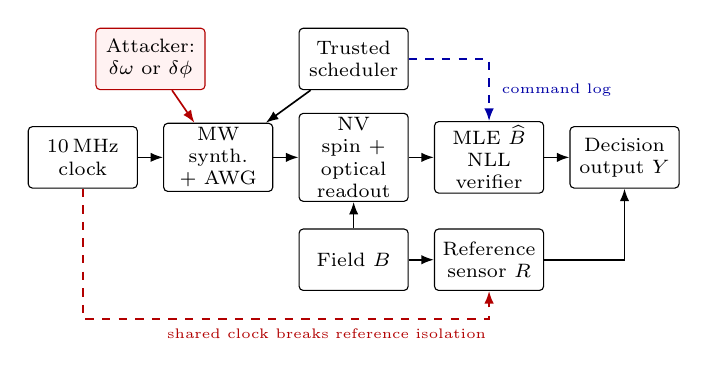
\begin{tikzpicture}[
  blk/.style={draw,rounded corners=1.5pt,align=center,font=\scriptsize,
              minimum height=0.78cm,text width=1.28cm,inner sep=1.5pt,fill=white},
  atk/.style={blk,draw=red!70!black,fill=red!5},
  flow/.style={-{Latex[length=1.6mm]},semithick},
  meta/.style={flow,dashed,blue!65!black},
  x=1cm,y=1cm]
\node[blk] (clk) at (0,0) {10\,MHz\\clock};
\node[blk] (syn) at (1.72,0) {MW synth.\\+ AWG};
\node[blk] (nv) at (3.44,0) {NV spin +\\optical readout};
\node[blk] (est) at (5.16,0) {MLE $\widehat B$\\NLL verifier};
\node[blk] (dec) at (6.88,0) {Decision\\output $Y$};
\node[atk] (atk) at (0.86,1.25) {Attacker:\\$\delta\omega$ or $\delta\phi$};
\node[blk] (sch) at (3.44,1.25) {Trusted\\scheduler};
\node[blk] (fld) at (3.44,-1.3) {Field $B$};
\node[blk] (ref) at (5.16,-1.3) {Reference\\sensor $R$};
\draw[flow] (clk) -- (syn);
\draw[flow] (syn) -- (nv);
\draw[flow] (nv) -- (est);
\draw[flow] (est) -- (dec);
\draw[flow] (sch) -- (syn);
\draw[meta] (sch) -| (est);
\node[font=\tiny,text=blue!65!black,anchor=west] at (5.2,0.85) {command log};
\draw[flow,red!70!black] (atk) -- (syn);
\draw[flow] (fld) -- (nv);
\draw[flow] (fld) -- (ref);
\draw[flow] (ref) -| (dec);
\draw[flow,dashed,red!70!black] (clk.south) -- (0,-2.05)
  -| node[pos=0.3,below,font=\tiny]{shared clock breaks reference isolation} (ref.south);
\end{tikzpicture}

\caption{Sensor chain and trust boundaries. The attacker offsets the drive frequency ($\delta\omega$)
or phase ($\delta\phi$) after the trusted scheduler. The reference is secure only if it shares no
clock, synthesizer or data path with the primary chain (red dashed).}
\label{fig:chain}
\end{figure}

The attacker's lever is the part of the chain that turns commands into microwave pulses
(Fig.~\ref{fig:chain}). A trusted scheduler chooses the interrogation time $t_k$ and analysis
phase $\phi_k$ of each setting $k$ and logs them. The synthesizer and AWG drive one NV transition,
and the estimator computes a field estimate $\Bhat$ from the photon counts and the logged commands. A verifier scores settings held out from the fit, and an optional reference
sensor supplies an independent reading $R$ of the same field. The decision stage combines them
into the released output $Y$.

The attacker acts between the scheduler and the spin. It can add a constant offset to the drive
frequency, or change the analysis phase of each pulse, either from a table prepared in advance or
with real-time knowledge of the schedule. It cannot observe the true field or the reference, and
it cannot alter counts, logs, software or the reference path. Such access would bypass any measurement check and calls for data-path protection instead.

We judge a defense by what it releases, not by how often it alarms. Table~\ref{tab:setup} defines
the measures. A release is \emph{harmful} if it misses the true field by more than 25\,nT, while the
attacker aims to shift the estimate by 100\,nT without an alarm; both values are evaluation
parameters, not operational standards. Because a defense can avoid harm by releasing nothing, we
also report coverage and the error of released outputs. With these measures, we can ask what the
primary sensor can detect on its own.

\begin{table}[t]
\centering
\caption{Measures and simulation settings of the frozen run.}
\label{tab:setup}
\footnotesize
\setlength{\tabcolsep}{3pt}
\renewcommand{\arraystretch}{1.1}
\begin{tabular}{@{}>{\raggedright\arraybackslash}p{0.23\columnwidth}>{\raggedright\arraybackslash}p{0.74\columnwidth}@{}}
\toprule
Harm & Fraction of attempts with released $|Y-B|>\epsilon_H=25$\,nT \\
Coverage & Fraction of attempts that release an output \\
RMSE & Root-mean-square error of released outputs \\
Alarm budget $\alpha$ & Fraction of clean sequences allowed to raise an alarm; 1\% \\
\midrule
Ramsey model & Eq.~\eqref{eq:ramsey}: $\Ttwo=100\,\mu$s, $\eta=0.1$, $c=1$; phases $0,\pi/2$ \\
Schedules & Fixed $t\in\{5,10,20,40,60\}\,\mu$s, or secret $t\sim U[5,60]\,\mu$s per setting \\
Sequence & 20 settings $\times$ 1000 shots (half fit, half verify); $B\sim U[0,1.9]\,\mu$T \\
Calibration & 4{,}096 clean sequences per pipeline; thresholds are empirical quantiles \\
Intervals & 95\% bootstrap over whole pipelines (10{,}000 draws; 2{,}000 post hoc) \\
Attacker table & Differential evolution, 4 starts $\times$ 30 members $\times$ 24 generations; 64/128 training/validation sequences; offsets in $\pm\pi$ \\
Spin-1 check & NV $S{=}1$, $^{14}$N $I{=}1$; hyperfine $-2.14$/$-2.70$\,MHz, quadrupole $-4.95$\,MHz; 25\,ns pulses, 10\,MHz Rabi, no RWA; $B_0=5,10,20$\,mT \\
\bottomrule
\end{tabular}
\end{table}

\section{Can the Sensor Detect the Attack on Its Own?}
\label{sec:primary}

A Ramsey sequence turns the field into a phase and the phase into a spin population. The first microwave pulse creates a superposition, and the spin then precesses for a time $t$ at a
rate set by its detuning from the drive. The second pulse, with analysis phase $\phi$, converts the
accumulated phase into a population that the optical readout measures. The probability of reading
the $m_s=0$ state is~\cite{degen2017quantum,rondin2014magnetometry}
\begin{equation}
 p=\tfrac12\bigl[1+(1-2\eta)\,c\,e^{-t/\Ttwo}\cos\Theta\bigr],\quad
 \Theta=(\gamma B+\delta\omega)t+\beta-\phi,
 \label{eq:ramsey}
\end{equation}
where $\gamma$ is the gyromagnetic ratio, $B$ the field and $\delta\omega$ any detuning of the drive.
The preparation phase is $\beta$, the contrast $c$, the dephasing time $\Ttwo$, and $\eta$ a symmetric
readout error. Repeating each setting $N$ times gives binomially distributed photon counts.

\textbf{Frequency offsets are undetectable.} The physics here is standard; its consequence for the
control chain is the point. Equation~\eqref{eq:ramsey} depends on the field and the drive only
through their sum $\gamma B+\delta\omega$. An attacker who lowers the drive
frequency by $\gamma\Delta B$ therefore produces exactly the count distribution of a field
$B+\Delta B$. This holds for any pulse shape and any schedule, including secret ones, as long as
the dynamics of the addressed transition depend on the field only through this detuning. Because
the clean and attacked data have the same distribution, every test computed from the primary
sensor's data raises an alarm with the same probability in both cases. In the terms of
cyber-physical security, the attack is \emph{undetectable}: its measurements are exactly those of a
legitimate state~\cite{pasqualetti2013attack}.

The equivalence is exact only in the two-level model, so we checked the neglected physics.
Equation~\eqref{eq:ramsey} ignores the second, unaddressed NV transition, the counter-rotating part
of the drive, and the $^{14}$N nuclear spin. We simulated the full coupled electron-nuclear system (Table~\ref{tab:setup}) at eight random
settings per bias field. The largest difference between the populations under a real field
change and under the equivalent drive offset was \SpinNominalDiff{}$\times10^{-4}$ at a 10\,mT bias
field and \SpinMaxDiff{}$\times10^{-4}$ at 5\,mT. For comparison, the spoof itself changes the
population by a median of \SpinSignal{}, and shot noise at 1000 shots is \SpinShotNoise{} per
setting. If the residual stays at this level, even an ideal detector that knew it exactly would
need at least \DetectSequencesNominal{} sequences at 10\,mT (\DetectSequencesWorst{} at 5\,mT) to
detect it with 50\% probability at a 1\% false-alarm rate. The attack is therefore undetectable
within any single sequence. Can the defender do better by hiding the schedule?

\textbf{Secret timing stops only precomputed phase attacks.} A phase actuator imitates a field
change only if it applies $\delta\phi_k=-\gamma\Delta B\,t_k$ with the true interrogation time.
If the defender draws each $t_k$ secretly, an attacker that committed to a table built for public
nominal times $t_{\rm nom}$ leaves a residual phase $\gamma\Delta B\,(t_{\rm nom}-t_k)$ that varies
from setting to setting. No single field value then explains all settings, and a likelihood test
on held-out settings detects the misfit. A frequency offset needs no knowledge of $t_k$, because the
extra phase grows with time automatically. Secret timing therefore does not help against it.

\textbf{Dual-transition driving cancels common clock errors.} The NV ground state offers a
hardware defense. It has two microwave transitions, $m_s=0\to+1$ and $m_s=0\to-1$, whose
frequencies move in opposite directions when the field changes:
$\omega_\pm=D\pm\gamma(B_0+B)$, where $D\approx2.87$\,GHz is the zero-field splitting and $B_0$
the bias field. A clock error, by contrast, shifts both drive tones in the same direction. Differencing the two measured detunings keeps $2\gamma(B_0+B)$ and cancels offsets common to both
tones, including drifts of $D$~\cite{fang2013quantumbeats,bauch2018ultralong,hart2021dq}. A fractional clock
error $\epsilon$ scales both tones. At $\epsilon=1$\,ppm and $B_0=10$\,mT it biases a
single-transition estimate by about \ClockSingleBias{}\,nT but a dual-transition estimate by only
\ClockDualBias{}\,nT, forcing the attacker to inject a precise differential offset on two tones.
This is an algebraic bound, not a demonstrated defense. A single-transition sensor therefore needs
help from outside the chain; how much can an external reference provide?

\section{Can a Reference Sensor Restore the Estimate?}
\label{sec:reference}

\textbf{Two checks raise the alarm.} Each sequence splits its settings into an estimation set, on
which the maximum-likelihood estimate $\Bhat$ is fitted, and a verification set. The first check,
$S_N$, is the negative log-likelihood of the verification counts under $\Bhat$; it grows when the
data do not fit a single field. The second check, $S_R=|\Bhat-R|$, compares the primary estimate
with the reference reading. The defender first fixes a false-alarm budget $\alpha$, the fraction of
clean sequences allowed to raise an alarm; we use $\alpha=1\%$. Each check receives half of the
budget: its threshold is set so that only a fraction $\alpha/2$ of its scores on clean calibration
sequences lie above it~\cite{angelopoulos2023conformal}. The alarm fires when either check exceeds
its threshold, so on clean data it fires on at most $\alpha$ of sequences. We call the discrepancy
threshold $\kappa$.

\textbf{The reference is only useful if it is isolated.} Ideally, the reference measures the same
field through its own electronics, so the attack cannot reach it. In practice, it may share a clock
or synthesizer with the primary sensor, or carry an uncorrected calibration offset. This matters
because whatever the reference shares with the primary chain, the attacker can shift too. We model
the reading as
\begin{equation}
 R=B+b_R+\lambda\Delta B+\varepsilon,\qquad \varepsilon\sim\mathcal N(0,\sigma_R^2),
 \label{eq:reference}
\end{equation}
where $\sigma_R$ is the reference noise, $b_R$ a calibration offset, and $\lambda$ the fraction of
the spoof $\Delta B$ that also reaches the reference. An independent reference has $b_R=\lambda=0$.
A second NV sensor driven from the same clock has $\lambda=1$.

\textbf{Output policies.} Once the alarm is decided, the decision stage chooses what to release.
\emph{Fallback} releases $R$ on alarm and $\Bhat$ otherwise. \emph{Abstention} releases $\Bhat$
only without an alarm and releases nothing otherwise. \emph{Always-reference} ignores the primary
sensor. \emph{Fusion} rules blend the two sensors instead of switching. Inverse-variance fusion
releases $R+w(\Bhat-R)$ with $w=\sigma_R^2/(\sigma_R^2+\sigma_P^2)$, weighting each sensor by its
precision, where $\sigma_P$ is the primary sensor's clean error. Gated fusion uses fallback on alarm
and inverse-variance fusion otherwise. Clipped fusion releases $R+\mathrm{clip}(\Bhat-R,\pm\kappa)$,
so it follows the primary sensor only within the alarm threshold. Which of these policies limits
harm under attack?

\textbf{The reference sets a floor.} A fallback release is harmless only if the released sensor is
accurate. When the spoof makes $\Bhat$ harmful, only a released, accurate $R$ can avoid harm, so
fallback harm is at least the reference's own harm rate, whatever the alarm rule. For an
independent reference with Gaussian noise, that rate is $2\Phi(-\epsilon_H/\sigma_R)$, where
$\Phi$ is the standard normal cumulative distribution function. This is the probability that the
reference alone misses the true field by more than $\epsilon_H$. The same floor holds in the worst case for every rule of the form $Y=R+g(\Bhat-R)$ with any
function $g$. This class includes fallback, all fusion rules above, and any alarm on $\Bhat-R$. It assumes that the attacker chooses the spoof size without bound and that the reference error is
Gaussian and independent of the spoof. It also assumes that the primary error depends on neither
the field nor the spoof, and that the defender uses no prior on the field. Under these conditions $\Bhat$
carries no usable information about $B$. Rules that exploit a bounded field prior are outside this
statement. A floor is only a lower bound, though. How close does fallback get to it?

\textbf{Design equation.} Assume the spoof shifts the primary estimate by exactly $d>h$, with
$h=\epsilon_H$, and neglect the primary sensor's own noise, which is small next to the reference's.
The reference then reads $R=B+s+\varepsilon$ with shift $s=b_R+\lambda d$. Harm arises in two
disjoint ways, which give the two terms of
\begin{equation}
 H_F(d)=P(|s+\varepsilon|>h)+P\bigl(|s+\varepsilon|\le h,\ |d-s-\varepsilon|\le\kappa\bigr).
 \label{eq:closed}
\end{equation}
The first term covers an inaccurate reference: the released value is harmful whether or not the
alarm fires, because both sensors are wrong. The second term covers an accurate reference that
still leaves the discrepancy $|\Bhat-R|$ below $\kappa$. No alarm fires, so the spoofed $\Bhat$ is
released.

For an independent reference ($s=0$), the discrepancy is close to $d$, and the second term
separates three regimes of spoof size:
\begin{itemize}
\item \emph{Blind window}, $h<d\le\kappa-h$. The spoof is large enough to be harmful but too small
to push an accurate reference past the threshold. Every accurate reference is silent, so harm
is 1.
\item \emph{Transition region}, $\kappa-h<d<\kappa+h$. The alarm fires for some reference noise
values and not others, so harm falls as $d$ grows. This region matters because moderate spoofs
land here and are only partly caught.
\item \emph{Floor}, $d\ge\kappa+h$. Every accurate reference raises the alarm, so only the first
term remains.
\end{itemize}
Because the discrepancy can deviate in
either direction, its check is two-sided: the budget $\alpha/2$ is split equally between large
positive and large negative discrepancies. This gives
\begin{equation}
 \kappa\approx z_{1-\alpha/4}\sqrt{\sigma_R^2+\sigma_P^2},
 \label{eq:kappa}
\end{equation}
where $z_{1-\alpha/4}=\TheoryZ$ is the standard normal quantile. The blind window exists whenever
$\kappa>2h$. With the simulated primary noise $\sigma_P\approx\TheorySigmaPrimary$\,nT, this happens
once $\sigma_R>\TheorySigmaCritical$\,nT. At $\sigma_R=20$\,nT, spoofs from 25 to
\TheoryBlindUpper\,nT pass unnoticed. Equations~\eqref{eq:closed} and~\eqref{eq:kappa} thus become a
sizing rule for the reference. The next section tests them.

\section{Evaluation}
\label{sec:eval}

\textbf{Data sources.} Every result comes from a single simulation run whose cases, policies,
endpoints and random seeds were fixed and time-stamped before it ran, which we call the frozen run.
Two analyses added afterwards are marked post hoc: the design-equation comparison
(Fig.~\ref{fig:theory}) and the fusion replay (Table~\ref{tab:fusion}), which re-evaluates output rules
on the stored records without new simulation. The spin-1 simulation and clock arithmetic of
Sections~\ref{sec:intro}--\ref{sec:primary} are separate calculations.

\textbf{Setup.} Each pipeline calibrates its thresholds on its own clean sequences
(settings in Table~\ref{tab:setup}), taking the empirical quantile that leaves $\alpha/2$ of scores above
it, and fits its own attacker table. The defender uses a fixed public schedule, the same schedule with random analysis phases, or
secret times; each is a separate case, so the benefit of secrecy can be isolated. The run
contains 20 cases. Attack cases vary the actuator (phase or frequency), the schedule, and the
attacker's knowledge of the actual times. Reference-stress cases vary $\sigma_R\in\{5,15,50\}$\,nT,
add a 10\,nT offset or a shared fraction $\lambda\in\{0.5,1\}$, or shrink the spoof to 50\,nT.
Control cases include no attack, a genuine 100\,nT field change, and uncalibrated readout drift.
Thirty independently seeded pipelines, each with 512 clean/attacked pairs per case, give \TotalN{}
attempts per case and condition. Unless
stated otherwise, results
refer to the \emph{nominal configuration}: a 100\,nT frequency spoof, $\sigma_R=20$\,nT, and
thresholds calibrated at $\alpha=1\%$.

\textbf{Secret timing stops phase tables but not frequency offsets.} Table~\ref{tab:capability} reports how often each attack reaches its 100\,nT target without an
alarm, using only the likelihood check. In the disclosure rows, the attacker learns each actual time either before the 2\,$\mu$s its
actuator needs to apply the phase (timely) or after it (late); full knowledge gives the time
immediately. Mean-time and zero-offset tables are simple baselines for the optimized table. A nominal-time phase
attack succeeds on \FixedU{} of \TotalN{} attempts against the fixed schedule but on only
\HiddenU{} against secret times. Randomizing the analysis phase alone does not help, because the
attacker simply adds its offset to whatever phase is used. The attacker's strongest option against
secret times is a precommitted phase table: one phase offset per public nominal-time slot, chosen
by numerical optimization (differential evolution) on simulated data to shift the estimate while
still fitting the verifier. It shifts the estimate in \OptimizedT{} attempts but passes the verifier
in only \OptimizedU{}; since the search is finite, this is a lower bound on what a phase attacker
can do. A drive-frequency offset needs no schedule knowledge and succeeds on \FrequencyU{} of
\TotalN{} attempts even against secret times, with simulated count distributions matching the
field-shifted ones to within $\EquivalenceError$. With the primary sensor blind to this attack,
everything rests on the reference.

\begin{table}[t]
\centering
\caption{Attack capability, likelihood check only (frozen run, \TotalN{} attacks per row). Target:
100\,nT shift reached; undetected: without alarm. Detuning: frequency offset.}
\label{tab:capability}
\footnotesize
\begin{tabular}{@{}lrr@{}}
\toprule
Attack / defender schedule & Target & Undetected \\
\midrule
Nominal phase / fixed & 14{,}879 & 14{,}758 \\
Nominal phase / hidden phase & 14{,}669 & 14{,}593 \\
Nominal phase / hidden time & 2{,}569 & 1 \\
Late disclosure / hidden time & 2{,}569 & 1 \\
Timely disclosure / hidden time & 15{,}004 & 14{,}892 \\
Full knowledge / hidden time & 15{,}004 & 14{,}892 \\
Detuning / hidden time & 15{,}004 & 14{,}892 \\
Selected phase table / hidden time & 6{,}081 & 17 \\
Mean-time phase / hidden time & 5{,}900 & 14 \\
Zero offset / hidden time & 0 & 0

\\
\bottomrule
\end{tabular}
\end{table}

\textbf{Fallback reaches the floor, and the design equation explains it.} In the nominal
configuration, fallback releases a harmful estimate on \NominalHarmRate\% [\NominalHarmCI] of
attacks, the same rate as always-reference. This is the reference's own error rate at
$\sigma_R=20$\,nT, so no alarm rule can remove it. In a post-hoc comparison, the design equation reproduces this and every other tested condition
without fitting to attack data. Evaluated with the calibrated thresholds, it agrees with the observations within \TheoryMaxGap{} percentage points in all
\TheoryConditions{} reference conditions of the setup (Fig.~\ref{fig:theory}). The equation also explains the failures.
A 50\,nT spoof falls in the transition region and raises harm to \SmallHarmRate\%. A noisier
reference with $\sigma_R=50$\,nT widens $\kappa$ until even the 100\,nT spoof sits in the blind window,
and fallback harm rises to \WeakHarmRate\%, worse than the reference alone
(\WeakReferenceHarmRate\%). A precise reference with $\sigma_R=5$\,nT removes harm entirely. Reference
precision is one hardware requirement; isolation is the other.

\begin{figure}[t]
\centering
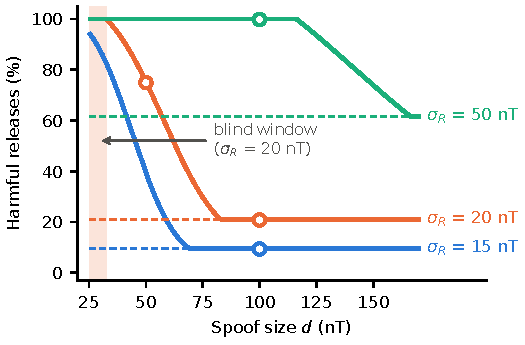
\includegraphics[width=\columnwidth]{figures/design_equation.pdf}
\caption{Fallback harm from Eq.~\eqref{eq:closed} (lines, post hoc), reference floors (dashed), and
frozen-run observations with 95\% intervals (circles). Shading: blind window at $\sigma_R=20$\,nT,
spoofs of 25--\TheoryBlindUpper\,nT that are harmful but raise no alarm.}
\label{fig:theory}
\end{figure}

\textbf{A shared clock defeats the reference.} Every departure from isolation in Eq.~\eqref{eq:reference} raises harm
(Table~\ref{tab:audit}). A reference that inherits the full spoof, as a second NV sensor on the same
clock would, releases harmful estimates on \FullHarmRate\% of attacks, yet alarms on only
\FullAlarmRate\%, because both sensors move together.

\begin{table}[t]
\centering
\caption{Reference dependency audit (frozen run): harmful releases of fallback under a 100\,nT
spoof, $\sigma_R=20$\,nT.}
\label{tab:audit}
\footnotesize
\setlength{\tabcolsep}{3pt}
\begin{tabular}{@{}llr@{}}
\toprule
Shared dependency & Model effect & Harm \\
\midrule
None (independent) & $b_R=\lambda=0$ & \NominalHarmRate\% \\
Calibration or offset error & $b_R=10$\,nT & \ObsBiasHarmRate\% \\
Partially coupled paths & $\lambda=0.5$ & \HalfHarmRate\% \\
Shared clock or synthesizer & $\lambda=1$ & \FullHarmRate\% \\
Shared data path/software & attacker rewrites $R$ & out of scope \\
\bottomrule
\end{tabular}
\end{table}

\textbf{What fallback, abstention and fusion buy.} If fallback cannot beat the reference under
attack, why use the primary sensor at all? The answer is clean precision. Without attack, fallback
releases the primary estimate most of the time, and its RMSE is \FallbackCleanRMSE\,nT, against
\ReferenceCleanRMSE\,nT for always-reference. The paired difference is \CleanDifference\,nT, with an
interval of [\CleanDifferenceCI] adjusted for multiple comparisons. This precision costs 20{,}000 primary shots per estimate, about \PrecessionSeconds\,s of free
precession with secret times before initialization and readout overheads. Reference integration time
and cost depend on the platform and are not modeled. The fusion replay in Table~\ref{tab:fusion} shows the price of pushing
precision further. Inverse-variance fusion is the most precise rule on clean data, but it trusts
the precise, compromised primary sensor and releases a harmful estimate on every attack. Gated and
clipped fusion fall in between, and every rule except always-reference has a worst case far above
the reference floor, which is only a lower bound.

Abstention trades availability for harm: it lowers harm by \ObsPFourDiff{} percentage points only
by cutting coverage under attack by \ObsPFiveDiff{} points. All \AbstainAttackH{} outputs it still releases are harmful, and each
release costs \AbstainShotsMillions{} million primary shots. Without attack, the alarm fires on \CleanAlarmRate\% [\CleanAlarmCI] of sequences, and a genuine
100\,nT field change raises only \GenuineAlarmCount{} alarms, because both sensors see it.

Averaging the reference is a cheaper route to precision if its errors are independent:
\TheoryAvgReadings{} readings give $\sigma_R=\TheoryAvgSigma$\,nT, matching fallback's clean precision
with a floor of \TheoryAvgFloor\%. Fallback pays off only if primary shots are far cheaper or drift prevents averaging.

\begin{table}[t]
\centering
\caption{Post-hoc replay of output rules (Section~\ref{sec:reference}) on frozen records,
$\sigma_R=20$\,nT. Worst case: model maximum over 0--300\,nT spoofs.}
\label{tab:fusion}
\footnotesize
\setlength{\tabcolsep}{3pt}
\begin{tabular}{@{}lrrrr@{}}
\toprule
& Clean & \multicolumn{2}{c}{Attacked harm (\%)} & Worst \\
Rule & RMSE (nT) & 100\,nT & 50\,nT & case (\%) \\
\midrule
Always reference & 19.98 & 20.78 & 20.78 & 21.2 \\
Combined fallback & 6.14 & 20.78 & 74.93 & 96.1 \\
Gated fusion & 6.09 & 20.78 & 74.93 & 95.4 \\
Inverse-variance fusion & 4.29 & 100.00 & 100.00 & 100.0 \\
Clipped fusion & 4.38 & 94.86 & 94.86 & 94.9

\\
\bottomrule
\end{tabular}
\end{table}

\section{Design Rules and Limitations}
\label{sec:rules}

The results reduce to four design rules, each with its hardware cost:
\begin{itemize}
\item \emph{Match the defense to the actuator.} Secret timing needs only a randomized scheduler;
it stops precomputed phase attacks, not frequency offsets.
\item \emph{Size the reference to the tolerance.} A 25\,nT tolerance needs
$\sigma_R<\TheorySigmaCritical$\,nT of total error, including drift and alignment.
\item \emph{Audit shared hardware.} The reference needs its own clock, synthesizer and data path;
sharing a clock gives \FullHarmRate\% harm.
\item \emph{Consider a dual-transition drive.} A second tone (synthesizer channel or IQ sideband)
should cancel common clock errors (\ClockSingleBias{} to \ClockDualBias{}\,nT per ppm, analytic);
it is untested against two-tone attacks.
\end{itemize}

These rules rest on simulation, not hardware. The Gaussian reference omits drift, bandwidth,
alignment, spatial mismatch and correlated noise, so a real reference must be characterized first.
The attacker is an ideal offset, not a circuit-level clock; its phase-table search is finite; the
pipelines share one code base; and full proofs of the floor exceed this paper.

\section{Conclusion}
\label{sec:conclusion}

In simulation, an NV Ramsey magnetometer cannot tell a sub-ppm drive offset from a field change. A reference restores integrity only down to its own error rate, only if precise enough to
close the blind window, and only if it shares no clock with the sensor. Next come circuit-level clock models, two-tone attacks, and NV hardware.

\bibliographystyle{IEEEtran}
\bibliography{references}

\end{document}
